\documentclass[]{tufte-handout}
\usepackage{amsmath,amssymb,amsthm}
\usepackage[pdftex]{graphicx}
\usepackage{listings}
\usepackage{color}

\definecolor{dkgreen}{rgb}{0,0.6,0}
\definecolor{gray}{rgb}{0.5,0.5,0.5}
\definecolor{mauve}{rgb}{0.58,0,0.82}

\lstset{frame=tb,
  language=Java,
  aboveskip=3mm,
  belowskip=3mm,
  showstringspaces=false,
  columns=flexible,
  basicstyle={\small\ttfamily},
  numbers=none,
  numberstyle=\tiny\color{gray},
  keywordstyle=\color{blue},
  commentstyle=\color{dkgreen},
  stringstyle=\color{mauve},
  breaklines=true,
  breakatwhitespace=true,
  tabsize=3
}


\title{COMP 210 \\ Lecture Notes 03 \\ Procedural Java}

\begin{document}
\maketitle

\begin{abstract}
In these notes we look at designing, implementing, and testing basic procedures in Java. We will rarely, perhaps never, program in this style with Java. It's not object-oriented. We're doing this as a Hello-World exercise. It lets us explore some key syntax in Java and see where it differs from C++ at the statement syntax level. It also lets us get started with JUnit, our new unit-testing framework.
\end{abstract}

\section{Procedures and Static Class Methods}

Java is not meant to be strictly procedural. You cannot even implement a procedure outside of bounds of a a class definition. There is, however, cause to have class methods that can be invoked without an object. These methods generally behave in the same fashion as a procedure\sidenote{we'll explore them in detail later} and certainly give us the ability to create the logical equivalent to the procedures we used in C++. These methods are called \textsc{static class methods}. The static keyword means their behavior is completely determined at compile time and they are therefore independent of any run-time values, specifically objects.

So, if you want to write procedural java you start with a class. You then implement all the procedures with the keywords \textit{public} and \textit{static}. The former ensures you can call the procedure from anywhere and the later indicates the the procedure is not a method relative to an instantiated object\sidenote{You'll see this in class an in the code that accompanies these notes}.

Without further ado, let's start cranking out some static class methods\sidenote{procedures}

\section{Functions}

Just like in C++, the parameter and return types are declared with the definition and checked by the compiler for consistency and correctness. The most important primitive types are the same: \textit{int} for integers, \textit{double} for double-precision floating point, \textit{char} for characters, and \textit{boolean}\sidenote{not just bool} for boolean values.

Unlike C++, we do not separate declaration and documentation from implementation. It all goes in one file. This is nice if you didn't like the separation but also makes it all to easy to skip early design steps and jump to implementation too quickly. So be warned.


Let's start with something that will cover a lot o basics: the classic recursive factorial. This lets us do a basic function that also calls a function, itself, and uses conditionals.

First we stub the function. In doing so we write out the complete header line. Eclipse can use this to kick start the documentation.

\begin{figure}
\begin{lstlisting}

public static int factorial(int n){
	return 0;
}

\end{lstlisting}
\caption{A Stub for \textit{factorial}}
\label{fig:funcStub}
\end{figure}

Now, if you're thinking that looks like C++, you're right. Java and C++ swim in the same syntax pool and draw from the same imperative paradigm. For basic statements in Java, what you want is pretty close to the equivalent C++. As we're getting started, just attempt some C++ and see if it flys.

To document this type \textit{/**} on the line above your stub and hit enter. Eclipse will get you started with annotations for the parameters and return types. We'll then add what we need. Here's the finished product.

\begin{figure}
\begin{lstlisting}

/**
 * Compute the factorial of n
 * @param n	 a positive integer
 * @return the factorial of n
 * @throws none
 * <dt><b>Precondition</b><dd>
 *    n >= 0
 * <dt><b>Postcondition</b><dd>
 *    none
 * <dt><b>Complexity</b><dd>
 *    Linear in n
 */
public static int factorial(int n){
	return 0;
}

\end{lstlisting}
\caption{Documentation for \textit{factorial}}
\label{fig:factDoxed}
\end{figure}

The usual suspects are all there. We begin with a purpose statement. The \@param tag documents each input and \@return documents the output.  The \@throws tag documents any exceptions generated by the procedure. The remaining documentation sections all use HTML to set them apart rather than an \@ annotation. This is because we're plugging into Java's documentation system and there is no \@pre, \@post, and \@complexity.  By using HTML, these sections will show up looking like the other documentation\sidenote{Go look these HTML tags up}. We'll see this in a little bit. Preconditions and postconditions are nothing new. Complexity is newer. We're going to start documented the complexity of our code. Sometimes you'll need to come back an fill this in after you've implmented the code because you're inventing a new solution. Other times you're implementing a known solution and can fill this in ahead of time. Either way, it should be there.

Now that the code is stubbed out and documented we can get to writing JUnit tests\sidenote{Go read \url{http://www.vogella.com/tutorials/JUnit/article.html} for a great write up JUnit}. In this case, we have no previously existing test file for our class so we need to generate one. Eclipse can really, really help you get started here. First we get to the New dialog\sidenote{File menu, quick button, right click package in tests folder} and find the \textit{JUnit Test Case}. Select this brings up the dialog you see in figure~\ref{fig:newtest}.  Here we want to be sure and 	properly set the source folder and package. This creates a class so you want to start the name with an uppercase letter. I tend to just append \textit{\_Tests} after the class name and I recommend you adopt something similar. Finally, fill in or select the \textit{Class Under} so that Eclipse knows what classes are being tested by this test case and hit \textit{Next}.

\vspace{.1in}
\begin{center}
\begin{figure}[!htb]
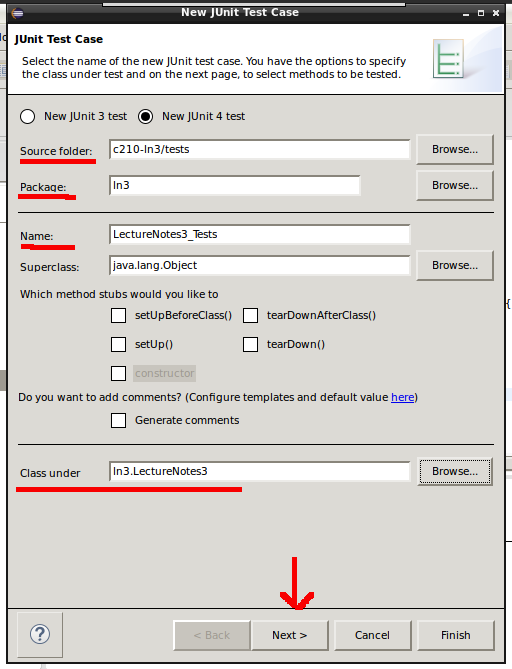
\includegraphics[scale=.5]{Eclipse-NewJUnitCase.png}
\caption{Dialog for JUnit Test Case Creation}
\label{fig:newtest}
\end{figure}
\end{center}
\vspace{.1in}

Hitting next brings up the dialog seen in figure~\ref{fig:selectstubs}. This lets you check off which methods you'd like Eclipse to stub out tests for. Notice I've already stubbed out the procedures we'll do later in these notes but have only checked \textit{factorial}. This capability makes a case for stubbing out all the methods you know for certain you need before this step as Eclipse can easily stub their tests all at once.

\vspace{.1in}
\begin{center}
\begin{figure}[!htb]
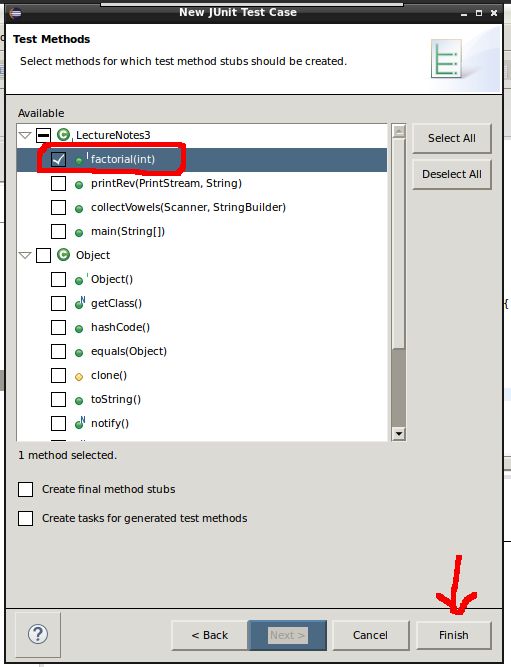
\includegraphics[scale=.5]{Eclipse-JUnitCaseStubSelect.png}
\caption{Dialog for JUnit Test Case Stub Selection}
\label{fig:selectstubs}
\end{figure}
\end{center}
\vspace{.1in}

Once you hit finish on the stub selection dialog you'll get a stub class like the one below.
\begin{figure}
\begin{lstlisting}

package ln3;

import static org.junit.Assert.*;

import org.junit.Test;

public class LectureNotes3_Tests {

	@Test
	public void testFactorial() {
		fail("Not yet implemented");
	}

}

\end{lstlisting}
\caption{Eclipse Generated JUnit Test Case for factorial}
\label{fig:testStub}
\end{figure}

This stub has a automatically failing test that's meant to remind you that you need to write these tests. There are also the requisite imports needed for basic testing. The \@Test annotation is detected by the compiler and is how Tests are recognized as such. \textit{It is not documentation, it's a compiler flag}.


You'll find some basic documentation for the possible assertions used in testing with JUnit at \url{https://github.com/junit-team/junit/wiki/Assertions}. We'll get a ton of mileage from \textit{assertEquals}. Eclipse has already written the import needed for us to avoid writing the complete ``path'' to the test like you see in the examples on the JUnit site. In our tests we'll leave off the optional error message as well and just state the expected and actual values\sidenote{Use them whenever you need or want though}.

\begin{figure}
\begin{lstlisting}

@Test
public void testFactorial() {
	assertEquals(1,LectureNotes3.factorial(0));
	assertEquals(1,LectureNotes3.factorial(1));
	assertEquals(2,LectureNotes3.factorial(2));
	assertEquals(120,LectureNotes3.factorial(5));
}

\end{lstlisting}
\label{fig:factTests}
\caption{JUnit Unit-Test for \textit{factorial}}
\end{figure}

Once again, it looks a lot like C++ doesn't it? Take note that to call the function, we start with the class name then use the dot operator, then the function name. Now, take a moment to hover the mouse over \textit{factorial}. You'll see why we used the HTML\@. Eclipse pulls up a nicely formatted version of your documentation. As programs get larger an span many many files, it's extremely helpful to have your documentation on hand as needed. You may also have noticed that Eclipse brings up an auto-correct box after you type the dot operator. This too is super nice. When you're using libraries this is nice chance to browse for that method you know you need whose name you can't remember.

To run your tests we go to the \textit{Run} menu and select \textit{Run As > JUnit Test}. Your tests will run. 	The results are displayed where the Package explore is. It's important to note that once a JUnit assertion fails, the test program stops.  In figure~\ref{fig:tests} you'll see only one failure report because the test stopped at the first failed assertion.

\vspace{.1in}
\begin{center}
\begin{figure}[!htb]
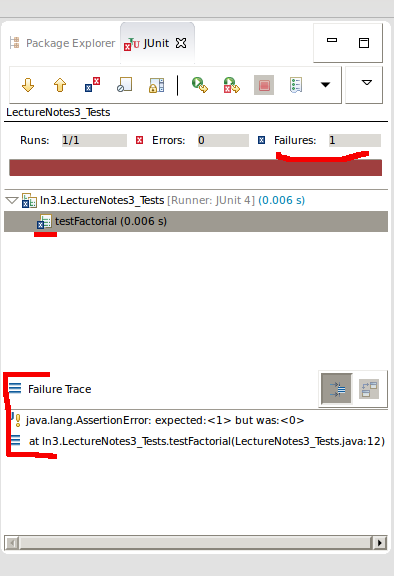
\includegraphics[scale=.5]{Eclipse-TestResult.png}
\caption{JUnit Test results with failed test}
\label{fig:tests}
\end{figure}
\end{center}
\vspace{.1in}

Ok. Implementation time. Once again, let's look at the finished product. It should look familiar. I'm leaving the documentation off to save space.

\begin{figure}
\begin{lstlisting}

/**
 * Documentation is here
 */
public static int factorial(int n){
	if ( n == 0 ){
		return 0;
	}
	else{
		return n * LectureNotes3.factorial(n-1);
	}
}

\end{lstlisting}
\label{fig:factorial}
\caption{Implementation for \textit{factorial}}
\end{figure}

We can see that basic operator syntax and if style conditionals in Java are exactly as they are in C++. As you typed this code you should have noticed things like braces matching happening automatically. Now re-run the tests and see that they pass.

\section{Output Procedures}

Java has streaming output just like C++ and we can use one type of stream to manage basic console and file output while using strings for testing. That type is \textit{PrintStream}\sidenote{\url{https://docs.oracle.com/javase/7/docs/api/java/io/PrintStream.html}}.

The problem we'll solve is to write a string backwards. This lets us make use of the Java String class as well as the PrintStream. Strings in Java are just a bit different than C++. We'll tease out the differences as needed. It's worth looking at the official tutorial\sidenote{\url{https://docs.oracle.com/javase/tutorial/java/data/strings.html}} in addition to the reference documentation.

First the documentation and stub.

\begin{figure}
\begin{lstlisting}

/**
 * Print the string str backwards on the stream out
 * @param out Stream where the reverse is written
 * @param str string to be printed in reverse
 * @throws none
 * <dt><b>Precondition</b><dd>
 *    none
 * <dt><b>Postcondition</b><dd>
 *    for non-empty str, it's contents are written (in reverse)
 * <dt><b>Complexity</b><dd>
 *   Linear in the size of str
 */
public static void printRev(PrintStream out, String str){

	return;
}

\end{lstlisting}
\label{fig:printrevdox}
\caption{Documentation and Stub for \textit{printRev}}
\end{figure}

Now the tests. Let's start with the finished product then break it down. Type these as is first. Eclipse will flag the the new types as errors because their classes have not be imported. If you right click the red-underlined test an option dialog pops up. One of the options is to add the import. This feature is very, very nice. It lets you code first and import as you go\sidenote{it will make more sense when you see and do it}. Just be sure you select the correct import.

\begin{figure}
\begin{lstlisting}

@Test
public void testPrintRev(){

	ByteArrayOutputStream actual = new ByteArrayOutputStream();
	LectureNotes3.printRev(new PrintStream(actual),"");
	assertEquals("",actual.toString());

	actual = new ByteArrayOutputStream();
	LectureNotes3.printRev(new PrintStream(actual),"hello");
	assertEquals("olleh",actual.toString());

}

\end{lstlisting}
\label{fig:printrevtests}
\caption{Unit-Tests for \textit{printRev}}
\end{figure}

The \textit{ByteArrayOutputStream} is a mutable stream that stores data in a ByteArray. This storage property is why we're using it. It will hold onto the text that our procedure adds to it. We can then access that data as a string with the \textit{toString} method.

Notice that every object is allocated dynamically using \textit{new}\sidenote{same meaning as in C++}. That's because \textit{every single object in Java is dynamically allocated on the heap}. The good news is there is no \textit{delete} because Java is \textsc{garbage collected}. As the program runs, the Java Virtual machine that executes the code will clean up the heap as needed. So, get used to dynamically allocating objects and treating those objects as \textit{class literals}.

There two other things to take note of here:
\begin{itemize}
\item In C++ we were using the C++11 curly brace initialization for all our variables. In Java, we use traditional assignment operator initialization. You can see this with the declaration and initialization of \textit{actual}.
\item String literals are done just as they are in C++.
\end{itemize}

Now the implementation. We'll use a for loop on this one. Notice it's just like in C++.

\begin{figure}
\begin{lstlisting}

public static void printRev(PrintStream out, String str){

	for( int i = str.length()-1 ; i >= 0; --i ){
		out.print(str.charAt(i));
	}

	return;
}

\end{lstlisting}
\label{fig:printrevimpl}
\caption{Implementation of \textit{printRev}}
\end{figure}

PrintStream objects print more or less like ostreams in C++ where \textit{out.print(\ldots)} acts a lot like \textit{out $<<$ \ldots}. There is also a \textit{println} method that adds a newline after printing automatically. It's incredibly useful. Now re-run those tests and see that this code works.

Now what about actual output? The standard output is \textit{System.out} in Java. So printing to the console just means printing to System.out.

\begin{figure}
\begin{lstlisting}
public static void main(String[] args){

	LectureNotes3.printRev(System.out,"racecar");
	System.println();

	return;
}
\end{lstlisting}
\label{fig:consoleOutput}
\caption{Output to the Standard Output PrintStream}
\end{figure}

The output procedure doesn't print a newline at the end so I've added the \textit{	System.println() } to do that and avoid console output ugliness.

\section{Input Procedures and Mutators}

Java is pass by value. You cannot pass a variable by reference so you cannot write mutators and input procedures like we did in C++. However, it is possible to pass a \textsc{mutable object} to a procedure, allow that procedure to mutate the object, and thereby get the the same end result. This is very subtle difference. Even when we switch to OOP we'll come up against it. You've actually seen this at work in the output procedure tests. The PrintStream object contained a mutable ByteArrayOutputStream which gets modified by the procedure. This was all done behind the scenes though.
\sidenote{ It's worth noting that primitive types are not class-based objects and we absolutely cannot mutate their variables by passing them to procedures or methods}.

When your goal is explicit mutation its important to know that you must work through a class' mutator methods. Assigning a new value to the procedure's parameter doesn't modify the passed argument, it just makes the local parameter reference a new, different object. This is equivalent to allocating a new object on a non-reference pointer in C++. The address of new data is assigned to local data only and doesn't change the value of the passed argument. The following code illustrates the difference in psuedo-Java.

\begin{figure}
\begin{lstlisting}
public void foo(SomeType var, ...){

  // Assign new value to local variable var
  var = new SomeType(...);

  // Modify existing value of var via mutator method
  var.setSomeTypeField(...);
}
\end{lstlisting}
\label{fig:mutatable}
\caption{Mutation via mutators vs the assignment operator}
\end{figure}

We'll kill two birds with one stone and look at mutation in the context of an input procedure. The procedure in question will read a stream character by character and keep all the vowels. Those vowels should be added to a string in the order in which they were read from a string. This seems straight forward enough but there are a few hoops we'll have to jump through to make this work in Java.

The basic String class in Java provides an immutable string. For mutable strings you can use the \textit{StringBuilder} \sidenote{\url{https://docs.oracle.com/javase/7/docs/api/java/lang/StringBuilder.html}} class. Thankfully \textit{every single Java class has a \textit{toString} method that returns a string representation of the object} and for StringBuilder objects that string is the \textit{String} type equivalent of the built string. Getting from StringBuilder to String is super easy. The reverse is easy as well. StringBuilders have a String based constructor as well.

Our replacement for \textit{istream} and basic input streams will be \textit{Scanner} objects\sidenote{\url{https://docs.oracle.com/javase/7/docs/api/java/util/Scanner.html}}. Scanners read almost all the primitive types, allow the programmer to choose a delimiter for tokens, and can be used in conjunction with files, the standard input, and strings. The one primitive type they do not do is characters, the type we want for our problem. The fix is simple enough though, read in data a String at a time, and then iterate through the string one character at a time.

Ok. Let's get to it. First the documentation and stub.

\begin{figure}
\begin{lstlisting}

/**
 * Read in all the vowels from in and write them in order
 *  to vowels.
 * @param in Scanner for the input stream
 * @param vowels StringBuilder where vowels from in are
 *   written
 * @throws
 * <dt><b>Preconditions</b><dd>
 *   none
 * <dt><b>Postconditions</b><dd>
 *   Consumes all characters in Scanner in
 * <dt><b>Complexity</b><dd>
 *   Linear in the number characters in Scanner in
 */
public static void collectVowels(Scanner in, StringBuilder vowels){

	return;
}

\end{lstlisting}
\label{fig:vowelsdox}
\caption{Documentation and Stub for \textit{collectVowels}}
\end{figure}

Now tests. Notice the liberal use of unnamed, dynamically allocated Scanners\sidenote{ \textit{new Foo(\ldots)} is the new literal}.

\begin{figure}
\begin{lstlisting}

@Test
public void testCollectVowels(){
	StringBuilder actual;

	actual = new StringBuilder("");
	LectureNotes3.collectVowels(new Scanner(""), actual);
	assertEquals("",actual.toString());

	actual = new StringBuilder("");
	LectureNotes3.collectVowels(new Scanner("ab c d efg432"), actual);
	assertEquals("ae",actual.toString());
}

\end{lstlisting}
\label{fig:vowelstests}
\caption{Unit-Tests for \textit{collectVowels}}
\end{figure}

Now for the implementation. The \textit{while} loop makes sense because we don't know how many tokens are in the stream and cannot count through them. On the other hand, we can count through the String's characters and a for loop works just fine there. Finally, notice boolean arithmetic is strictly binary, just like C++.

\begin{figure}
\begin{lstlisting}
public static void collectVowels(Scanner in, StringBuilder vowels){

	while( in.hasNext() ){
		String nxt_line = in.next();
		for(int i = 0; i < nxt_line.length(); i++){
			char nxt_char = nxt_line.charAt(i);
			if( nxt_char == 'a' || nxt_char == 'i' ||
				nxt_char == 'e' || nxt_char == 'o' ||
				nxt_char == 'u'){

				// Mutator!
				vowels.append(nxt_char);
			}
		}
	}

	return;
}
\end{lstlisting}
\label{fig:vowelsimpl}
\caption{Implementation of \textit{collectVowels}}
\end{figure}

To run this on console/CLI input we construct a Scanner on \textit{System.in}, the standard input. In linux, Ctrl-D will send the end of file/stream character/signal to the computer. So when you run this, press Ctrl-D to terminate console input.

\begin{figure}
\begin{lstlisting}
public static void main(String[] args) {

	LectureNotes3.printRev(System.out, "racecar");
	System.out.println();

	StringBuilder vowels = new StringBuilder("");
	LectureNotes3.collectVowels(new Scanner(System.in),vowels);

	System.out.println(vowels.toString());

	return;
}
\end{lstlisting}

\label{fig:cliInput}
\caption{Using System.in Scanners for Console Input}
\end{figure}
\section{Don't Try this At Home}

Once again. This is not the mode in which you should be using Java. We might design and implement procedures, but it will always be in support of a larger Class-based design. That being said, we will design functional class methods, class I/O methods, and class mutator and the general approach is them same for them as it is for their procedural counter parts. We're starting here to get our feet with Eclipse and JUnit while working with some basic statement-level Java. If you've been playing along, then go tinker. You'll have some fresh procedures to design and implement for lab 1.

\end{document}
